\documentclass[20pt,landscape,a4paper]{foils}
\usepackage[utf8]{inputenc}
\usepackage[T1]{fontenc}
\usepackage{helvet}
\renewcommand{\familydefault}{\sfdefault}
\usepackage[margin=0.6in,headheight=0.5in,headsep=0.15in,footskip=0.35in]{geometry}
\usepackage[table]{xcolor}
\usepackage{amsmath,amssymb}
\usepackage{booktabs}
\usepackage{tabularx}
\usepackage{array}
\usepackage{tcolorbox}
\tcbuselibrary{skins,breakable}
\usepackage{tikz}
\usetikzlibrary{positioning,calc,shapes.geometric,backgrounds,patterns}
\usepackage{fontawesome5}
\usepackage{enumitem}
\usepackage{multicol}
\usepackage{hyperref}

% --- Color Palette Definition ---
\definecolor{NavyPrimary}{HTML}{0F2C59}
\definecolor{TealAccent}{HTML}{008080}
\definecolor{AmberAccent}{HTML}{D97706}
\definecolor{SlateLight}{HTML}{F8FAFC}
\definecolor{SlateBorder}{HTML}{CBD5E1}
\definecolor{CharcoalText}{HTML}{1E293B}
\definecolor{CardBg}{HTML}{FFFFFF}

\hypersetup{
    colorlinks=true,
    linkcolor=NavyPrimary,
    urlcolor=TealAccent
}

% --- FoilTeX Header & Footer Setup ---
\MyLogo{\textcolor{NavyPrimary}{\small\faServer~ \textbf{Nexa AI Platform}}}
\Restriction{\textcolor{TealAccent}{\small\faLock~ \textbf{Confidential}}}

% --- Custom tcolorbox Styles ---
\tcbset{
    basebox/.style={
        enhanced,
        arc=4pt,
        boxrule=1pt,
        colback=CardBg,
        colframe=SlateBorder,
        boxsep=6pt,
        top=6pt,bottom=6pt,left=10pt,right=10pt
    },
    headerbox/.style={
        enhanced,
        arc=5pt,
        boxrule=0pt,
        colback=NavyPrimary,
        coltext=white,
        boxsep=8pt,
        top=8pt,bottom=8pt,left=14pt,right=14pt
    },
    accentbox/.style={
        enhanced,
        arc=4pt,
        boxrule=1.5pt,
        colback=SlateLight,
        colframe=TealAccent,
        boxsep=8pt,
        top=8pt,bottom=8pt,left=10pt,right=10pt
    },
    amberbox/.style={
        enhanced,
        arc=4pt,
        boxrule=1.5pt,
        colback=SlateLight,
        colframe=AmberAccent,
        boxsep=8pt,
        top=8pt,bottom=8pt,left=10pt,right=10pt
    }
}

% --- Custom Command for Slide Cards ---
\newcommand{\SlideHeader}[2]{%
  \begin{tcolorbox}[headerbox]
    {\Huge\bfseries #1} \hfill {\large\textcolor{SlateBorder}{#2}}
  \end{tcolorbox}
  \vspace{6pt}
}

\begin{document}

% ==========================================
% SLIDE 1: TITLE SLIDE
% ==========================================
\begin{tcolorbox}[enhanced, arc=8pt, boxrule=2pt, colback=NavyPrimary, colframe=TealAccent, boxsep=16pt, top=18pt, bottom=18pt]
  \centering
  \textcolor{AmberAccent}{\Huge \faRocket~ \textbf{NEXA ENTERPRISE AI PLATFORM}} \par
  \vspace{10pt}
  {\color{white}\Huge\bfseries High-Readability Architecture \& Deployment} \par
  \vspace{8pt}
  {\color{SlateBorder}\Large Scalable Model Serving, Quantization Dynamics, and Zero-Trust Guardrails} \par
  \vspace{18pt}
  \begin{tcolorbox}[enhanced, colback=white!10, colframe=white!30, arc=4pt, width=0.85\textwidth, halign=center]
    {\color{white}\large \textbf{Presenters:} Dr. Marcus Vance \& Dr. Elena Rostova} \par
    \vspace{4pt}
    {\color{SlateBorder}\small Nexa Systems Innovation Labs \quad|\quad Enterprise Seminar Series 2026}
  \end{tcolorbox}
\end{tcolorbox}
\pagebreak

% ==========================================
% SLIDE 2: WORKSHOP AGENDA
% ==========================================
\SlideHeader{Workshop Agenda}{Overview of Key Technical Modules}

\noindent
\begin{minipage}[t]{0.48\textwidth}
  \begin{tcolorbox}[accentbox, title={\textcolor{NavyPrimary}{\large \faCogs~ \textbf{Module 01: Core Architecture}}}, fonttitle=\bfseries]
    \begin{itemize}[leftmargin=16pt, label=\textcolor{TealAccent}{\small\faCheck}]
      \item Distributed Neural Data Ingestion
      \item High-Speed Tokenization Pipelines
      \item Hierarchical HNSW Vector Indexing
    \end{itemize}
  \end{tcolorbox}
\end{minipage}%
\hfill
\begin{minipage}[t]{0.48\textwidth}
  \begin{tcolorbox}[accentbox, title={\textcolor{NavyPrimary}{\large \faServer~ \textbf{Module 02: High-Throughput Serving}}}, fonttitle=\bfseries]
    \begin{itemize}[leftmargin=16pt, label=\textcolor{TealAccent}{\small\faCheck}]
      \item FP16 vs INT8 vs INT4 Benchmarks
      \item Continuous Batching \& KV-Cache
      \item Memory Footprint \& Latency Profiling
    \end{itemize}
  \end{tcolorbox}
\end{minipage}

\par\vspace{6pt}

\noindent
\begin{minipage}[t]{0.48\textwidth}
  \begin{tcolorbox}[amberbox, title={\textcolor{NavyPrimary}{\large \faLock~ \textbf{Module 03: Zero-Trust Safety}}}, fonttitle=\bfseries]
    \begin{itemize}[leftmargin=16pt, label=\textcolor{AmberAccent}{\small\faCheck}]
      \item Real-Time Input Guardrails \& PII Redaction
      \item Hallucination Mitigation Protocols
      \item Isolated Enclave Execution
    \end{itemize}
  \end{tcolorbox}
\end{minipage}%
\hfill
\begin{minipage}[t]{0.48\textwidth}
  \begin{tcolorbox}[amberbox, title={\textcolor{NavyPrimary}{\large \faChartLine~ \textbf{Module 04: Production Case Study}}}, fonttitle=\bfseries]
    \begin{itemize}[leftmargin=16pt, label=\textcolor{AmberAccent}{\small\faCheck}]
      \item Meridian Health 4.5M Note Deployment
      \item 99.999\% Uptime \& 42ms Latency Results
      \item Engineering Takeaways \& Checklist
    \end{itemize}
  \end{tcolorbox}
\end{minipage}
\pagebreak

% ==========================================
% SLIDE 3: SECTION 1 DIVIDER
% ==========================================
\vspace*{0.8cm}
\begin{tcolorbox}[enhanced, colback=SlateLight, colframe=NavyPrimary, boxrule=3pt, arc=6pt, boxsep=16pt]
  \textcolor{TealAccent}{\Large \textbf{SECTION 01}} \par\vspace{6pt}
  {\Huge\bfseries Core Architecture \& Data Engine} \par\vspace{10pt}
  \textcolor{CharcoalText}{\large Distributed storage, real-time tokenization, vector indexing, and pipeline resiliency.}
\end{tcolorbox}
\pagebreak

% ==========================================
% SLIDE 4: KEY PILLARS
% ==========================================
\SlideHeader{Key Pillars of Nexa AI Platform}{Engineered for Sub-10ms Latency \& Safety}

\noindent
\begin{minipage}[t]{0.31\textwidth}
  \begin{tcolorbox}[basebox]
    \centering
    \textcolor{TealAccent}{\Huge \faCogs} \par\vspace{6pt}
    {\large\bfseries Sub-10ms Core} \par\vspace{4pt}
    \small C++ inference kernel leveraging fused CUDA operators, shared KV-cache layers, and dynamic request batching for peak efficiency.
  \end{tcolorbox}
\end{minipage}%
\hfill
\begin{minipage}[t]{0.31\textwidth}
  \begin{tcolorbox}[basebox]
    \centering
    \textcolor{NavyPrimary}{\Huge \faLock} \par\vspace{6pt}
    {\large\bfseries Zero-Trust Enclave} \par\vspace{4pt}
    \small End-to-end payload encryption with hardware-attested secure enclaves preventing unauthorized data leaks.
  \end{tcolorbox}
\end{minipage}%
\hfill
\begin{minipage}[t]{0.31\textwidth}
  \begin{tcolorbox}[basebox]
    \centering
    \textcolor{AmberAccent}{\Huge \faLayerGroup} \par\vspace{6pt}
    {\large\bfseries Elastic Mesh} \par\vspace{4pt}
    \small Automated Kubernetes scaling across multi-cloud GPU nodes with dynamic load-balancing and zero-downtime failover.
  \end{tcolorbox}
\end{minipage}
\pagebreak

% ==========================================
% SLIDE 5: NEURAL DATA PIPELINE
% ==========================================
\SlideHeader{Neural Data Pipeline \& Ingestion}{High-Yield Processing of Unstructured Data}

\begin{itemize}[leftmargin=20pt, label=\textcolor{NavyPrimary}{\small\faCheck}]
  \item \textbf{Multi-Format Ingestion}: Native support for PDFs, HTML, tabular data, and raw audio streams.
  \item \textbf{Ultra-Fast Tokenization}: Rust-backed tokenizers processing over 500,000 tokens/sec per GPU node.
  \item \textbf{Hierarchical Vector Indexing}: Dual HNSW graphs with Product Quantization (PQ) for sub-millisecond search.
  \item \textbf{Automated Deduplication}: MinHash LSH filter delivering a 99.9\% clean data yield prior to model embedding.
\end{itemize}

\vspace{6pt}
\begin{tcolorbox}[accentbox]
  \textcolor{NavyPrimary}{\textbf{\faLightbulb~ Key Engineering Insight:}} \small Decoupling the ingestion pipeline from model inference nodes reduced vector store lock contention by 84\% during peak traffic windows.
\end{tcolorbox}
\pagebreak

% ==========================================
% SLIDE 6: TIKZ ARCHITECTURE DIAGRAM
% ==========================================
\SlideHeader{End-to-End System Architecture}{Distributed Pipeline Topology}

\centering
\begin{tikzpicture}[
    node distance=0.8cm and 0.6cm,
    block/.style={rectangle, draw=NavyPrimary, fill=SlateLight, thick, rounded corners=4pt, minimum width=2.5cm, minimum height=1.2cm, align=center, font=\small\bfseries},
    accentblock/.style={rectangle, draw=TealAccent, fill=TealAccent!10, thick, rounded corners=4pt, minimum width=2.6cm, minimum height=1.2cm, align=center, font=\small\bfseries},
    amberblock/.style={rectangle, draw=AmberAccent, fill=AmberAccent!10, thick, rounded corners=4pt, minimum width=2.6cm, minimum height=1.2cm, align=center, font=\small\bfseries},
    line/.style={draw=NavyPrimary, ->, >=stealth, ultra thick}
]

  % Nodes
  \node [block] (source) {\faDatabase\\ Data Sources\\ \tiny (PDFs, SQL, Logs)};
  \node [accentblock, right=of source] (ingest) {\faCogs\\ Ingestion Engine\\ \tiny (Rust Tokenizer)};
  \node [accentblock, right=of ingest] (vector) {\faLayerGroup\\ Vector Store\\ \tiny (HNSW + PQ)};
  \node [amberblock, right=of vector] (model) {\faServer\\ Model Cluster\\ \tiny (Nexa-70B INT8)};
  \node [block, right=of model] (gateway) {\faLock\\ API Gateway\\ \tiny (Safety Enclave)};

  % Arrows
  \draw [line] (source) -- (ingest);
  \draw [line] (ingest) -- (vector);
  \draw [line] (vector) -- (model);
  \draw [line] (model) -- (gateway);

  % Annotations
  \node [below=0.25cm of ingest, font=\tiny\color{CharcoalText}] {500k tok/s};
  \node [below=0.25cm of vector, font=\tiny\color{CharcoalText}] {Sub-1ms Query};
  \node [below=0.25cm of model, font=\tiny\color{CharcoalText}] {Continuous Batch};

\end{tikzpicture}

\vspace{6pt}
\begin{tcolorbox}[basebox]
  \small \textbf{Data Flow Summary:} Raw enterprise text is tokenized in real-time, matched against HNSW vector indexes, processed through quantized model clusters, and filtered via safety enclaves.
\end{tcolorbox}
\pagebreak

% ==========================================
% SLIDE 7: SECTION 2 DIVIDER
% ==========================================
\vspace*{0.8cm}
\begin{tcolorbox}[enhanced, colback=SlateLight, colframe=NavyPrimary, boxrule=3pt, arc=6pt, boxsep=16pt]
  \textcolor{TealAccent}{\Large \textbf{SECTION 02}} \par\vspace{6pt}
  {\Huge\bfseries High-Throughput Model Serving} \par\vspace{10pt}
  \textcolor{CharcoalText}{\large Quantization benchmarks, VRAM footprints, and batching optimizations.}
\end{tcolorbox}
\pagebreak

% ==========================================
% SLIDE 8: BENCHMARK TABLE
% ==========================================
\SlideHeader{Latency vs. Throughput Benchmarks}{Empirical Performance Across Model Variants}

\small
\begin{tabularx}{\textwidth}{X l c c c}
  \toprule
  \textbf{Model Variant} & \textbf{Quantization} & \textbf{VRAM Footprint} & \textbf{p99 Latency} & \textbf{Throughput} \\
  \midrule
  Nexa-70B-FP16 & Uncompressed (FP16) & 140 GB & 38 ms & 1,250 tok/s \\
  Nexa-70B-INT8 & AWQ INT8 (Recommended) & 72 GB & 22 ms & 2,400 tok/s \\
  Nexa-70B-INT4 & SmoothQuant INT4 & 38 GB & 14 ms & 4,100 tok/s \\
  Synapse-15B & FP16 Baseline & 30 GB & 11 ms & 5,800 tok/s \\
  Vertex-7B & AWQ INT8 & 8 GB & 6 ms & 12,500 tok/s \\
  \bottomrule
\end{tabularx}

\vspace{6pt}
\begin{tcolorbox}[accentbox]
  \small \textbf{Benchmark Takeaway:} AWQ INT8 quantization offers a 48.5\% reduction in VRAM requirement while nearly doubling throughput, with less than 0.15\% degradation on standard accuracy suites.
\end{tcolorbox}
\pagebreak

% ==========================================
% SLIDE 9: MEMORY FOOTPRINT & QUANTIZATION
% ==========================================
\SlideHeader{Quantization \& Memory Footprint Dynamics}{Maximizing Hardware Utilization}

\noindent
\begin{minipage}[t]{0.48\textwidth}
  \begin{tcolorbox}[basebox, title={\textcolor{NavyPrimary}{\large \faCogs~ \textbf{Precision Trade-offs}}}, fonttitle=\bfseries]
    \begin{itemize}[leftmargin=14pt, label=\textcolor{TealAccent}{\small\faCheck}]
      \item \textbf{FP16 Standard}: Maximum precision, high VRAM demand (140GB for 70B parameters).
      \item \textbf{AWQ INT8}: Optimal balance for enterprise deployments; minimal accuracy loss.
      \item \textbf{SmoothQuant INT4}: Edge-deployment ready; extreme memory savings.
    \end{itemize}
  \end{tcolorbox}
\end{minipage}%
\hfill
\begin{minipage}[t]{0.48\textwidth}
  \begin{tcolorbox}[amberbox, title={\textcolor{NavyPrimary}{\large \faChartLine~ \textbf{Resource Savings}}}, fonttitle=\bfseries]
    \centering
    \vspace{4pt}
    {\Huge\bfseries\textcolor{AmberAccent}{73\%}} \par
    {\small VRAM Footprint Reduction} \par\vspace{6pt}
    {\Huge\bfseries\textcolor{NavyPrimary}{$3.2\times$}} \par
    {\small Throughput Multiplication} \par\vspace{6pt}
    \small Maintains 100\% multi-turn conversational accuracy across 32k context windows.
  \end{tcolorbox}
\end{minipage}
\pagebreak

% ==========================================
% SLIDE 10: SECTION 3 DIVIDER
% ==========================================
\vspace*{0.8cm}
\begin{tcolorbox}[enhanced, colback=SlateLight, colframe=NavyPrimary, boxrule=3pt, arc=6pt, boxsep=16pt]
  \textcolor{TealAccent}{\Large \textbf{SECTION 03}} \par\vspace{6pt}
  {\Huge\bfseries Enterprise Security \& Governance} \par\vspace{10pt}
  \textcolor{CharcoalText}{\large Real-time guardrails, PII redaction, and compliance enforcement.}
\end{tcolorbox}
\pagebreak

% ==========================================
% SLIDE 11: ZERO-TRUST SAFETY
% ==========================================
\SlideHeader{Zero-Trust Safety \& Guardrails Architecture}{Comprehensive Threat Defense}

\noindent
\begin{minipage}[t]{0.48\textwidth}
  \begin{tcolorbox}[accentbox, title={\textcolor{NavyPrimary}{\large \faLock~ \textbf{Input Guardrails}}}, fonttitle=\bfseries]
    \begin{itemize}[leftmargin=14pt, label=\textcolor{TealAccent}{\small\faCheck}]
      \item \textbf{PII Masking}: Automatic regex and embedding-based sanitization before model entry.
      \item \textbf{Prompt Injection Defense}: 99.8\% detection rate against multi-turn jailbreaks.
      \item \textbf{Policy Enforcement}: Real-time context alignment checks against enterprise rules.
    \end{itemize}
  \end{tcolorbox}
\end{minipage}%
\hfill
\begin{minipage}[t]{0.48\textwidth}
  \begin{tcolorbox}[accentbox, title={\textcolor{NavyPrimary}{\large \faLock~ \textbf{Output Verification}}}, fonttitle=\bfseries]
    \begin{itemize}[leftmargin=14pt, label=\textcolor{TealAccent}{\small\faCheck}]
      \item \textbf{Hallucination Scoring}: Automated output confidence validation ($<1.2\%$ error rate).
      \item \textbf{Vector Fact Check}: Real-time verification against corporate knowledge bases.
      \item \textbf{Differential Privacy}: Noise injection to protect sensitive data queries.
    \end{itemize}
  \end{tcolorbox}
\end{minipage}
\pagebreak

% ==========================================
% SLIDE 12: SECTION 4 DIVIDER
% ==========================================
\vspace*{0.8cm}
\begin{tcolorbox}[enhanced, colback=SlateLight, colframe=NavyPrimary, boxrule=3pt, arc=6pt, boxsep=16pt]
  \textcolor{TealAccent}{\Large \textbf{SECTION 04}} \par\vspace{6pt}
  {\Huge\bfseries Production Case Study} \par\vspace{10pt}
  \textcolor{CharcoalText}{\large Meridian Health 4.5M clinical notes processing deployment.}
\end{tcolorbox}
\pagebreak

% ==========================================
% SLIDE 13: CASE STUDY - MERIDIAN HEALTH
% ==========================================
\SlideHeader{Production Deployment: Meridian Health}{Enterprise Healthcare Case Study}

\begin{tcolorbox}[basebox]
  \begin{description}[leftmargin=8pt]
    \item[\textcolor{NavyPrimary}{\textbf{Enterprise Challenge:}}] Processing 4.5 million patient clinical records daily under strict HIPAA compliance standards while reducing response latency.
    \item[\textcolor{TealAccent}{\textbf{Architectural Solution:}}] Deployed Nexa-70B AWQ INT8 inside isolated AWS GovCloud enclaves with hardware-backed security modules.
  \end{description}
\end{tcolorbox}

\vspace{6pt}
\noindent
\begin{minipage}[t]{0.31\textwidth}
  \begin{tcolorbox}[amberbox]
    \centering
    {\Huge\bfseries\textcolor{AmberAccent}{42ms}} \par\vspace{2pt}
    {\small Average Latency} \par
    \tiny (Reduced from 1,800ms)
  \end{tcolorbox}
\end{minipage}%
\hfill
\begin{minipage}[t]{0.31\textwidth}
  \begin{tcolorbox}[accentbox]
    \centering
    {\Huge\bfseries\textcolor{TealAccent}{64\%}} \par\vspace{2pt}
    {\small Infrastructure Savings} \par
    \tiny (vs. Legacy SaaS APIs)
  \end{tcolorbox}
\end{minipage}%
\hfill
\begin{minipage}[t]{0.31\textwidth}
  \begin{tcolorbox}[basebox]
    \centering
    {\Huge\bfseries\textcolor{NavyPrimary}{99.999\%}} \par\vspace{2pt}
    {\small System Availability} \par
    \tiny (12 Months Continuous Operation)
  \end{tcolorbox}
\end{minipage}
\pagebreak

% ==========================================
% SLIDE 14: WORKSHOP SUMMARY & TAKEAWAYS
% ==========================================
\SlideHeader{Workshop Summary \& Action Plan}{Key Engineering Takeaways for Production}

\noindent
\begin{minipage}[t]{0.48\textwidth}
  \begin{tcolorbox}[accentbox, title={\textcolor{NavyPrimary}{\large 1. Adopt INT8 Quantization}}]
    \small Halves hardware infrastructure cost without sacrificing response accuracy or conversational quality.
  \end{tcolorbox}
\end{minipage}%
\hfill
\begin{minipage}[t]{0.48\textwidth}
  \begin{tcolorbox}[accentbox, title={\textcolor{NavyPrimary}{\large 2. Decouple Data Ingestion}}]
    \small Separates vector embedding pipelines from model serving clusters to prevent I/O locking.
  \end{tcolorbox}
\end{minipage}

\par\vspace{6pt}

\noindent
\begin{minipage}[t]{0.48\textwidth}
  \begin{tcolorbox}[amberbox, title={\textcolor{NavyPrimary}{\large 3. Enforce Dual-Layer Safety}}]
    \small Implements pre-inference PII masking alongside post-inference hallucination scoring.
  \end{tcolorbox}
\end{minipage}%
\hfill
\begin{minipage}[t]{0.48\textwidth}
  \begin{tcolorbox}[amberbox, title={\textcolor{NavyPrimary}{\large 4. Continuous Profiling}}]
    \small Tracks p99 latency metrics and token throughput under real-world enterprise workloads.
  \end{tcolorbox}
\end{minipage}
\pagebreak

% ==========================================
% SLIDE 15: Q&A & CLOSING RESOURCES
% ==========================================
\SlideHeader{Questions \& Technical Resources}{Connecting with Nexa Engineering}

\noindent
\begin{minipage}[t]{0.58\textwidth}
  \begin{tcolorbox}[accentbox, title={\textcolor{NavyPrimary}{\large \faGlobe~ \textbf{Documentation \& Repositories}}}, fonttitle=\bfseries]
    \begin{itemize}[leftmargin=14pt, label=\textcolor{TealAccent}{\small\faCheck}]
      \item \textbf{Architecture Docs}: \href{https://docs.nexa-ai.internal/workshop}{docs.nexa-ai.internal/workshop}
      \item \textbf{GitHub Repository}: \href{https://github.com/nexa-labs/enterprise-ai-deck}{github.com/nexa-labs/enterprise-ai-deck}
      \item \textbf{Quantization Toolkit}: \href{https://github.com/nexa-labs/awq-quantizer}{github.com/nexa-labs/awq-quantizer}
    \end{itemize}
  \end{tcolorbox}
\end{minipage}%
\hfill
\begin{minipage}[t]{0.38\textwidth}
  \begin{tcolorbox}[amberbox, title={\textcolor{NavyPrimary}{\large \faEnvelope~ \textbf{Contact Leads}}}, fonttitle=\bfseries]
    \small
    \textbf{Dr. Marcus Vance} \par
    \texttt{m.vance@nexa-ai.internal} \par\vspace{4pt}
    \textbf{Dr. Elena Rostova} \par
    \texttt{e.rostova@nexa-ai.internal} \par\vspace{8pt}
    \centering
    \textcolor{NavyPrimary}{\large\bfseries Thank You!}
  \end{tcolorbox}
\end{minipage}

\end{document}
